\chapter{Representations of Trees}

There are many ways to represent static ordinal trees in memory.
The traditional way, which most people know and use, is to have a structure for each vertex pointing to all its children and its parent, and sometimes storing an additional value.
Each edge of the tree is stored twice as a pointer of size $w$.
Even if we did not need any other space to manage the vertex structures, the space occupied by the edges takes $\Omega (n \log n)$ bits.

In our discussion we assume that no additional value is present in vertices, and we are therefore interested in the structure of the tree itself.
If values are present, we could move them to an external table which is indexed by the number of the vertex to which it belongs.
This is one of the reasons why we will be interested in the \anyRank{} operations on tree.
This transformation maintains the same space complexity.

Let $\mathcal{T}(n)$ be a universe of all ordinal trees with $n$ vertices.
The size of the universe can be expressed using Catalan numbers:
$$ | \mathcal{T}(n) | = C_{n-1} = \frac{1}{n} {2n - 2 \choose n - 1}. $$
We saw a similar bound for balanced bit string, that is not a coincidence, as there exists a bijection between trees and balanced bit strings.
The difference of $-1$ stems from the fact that we are representing a tree with $n$ vertices rather than a forest of trees containing $n$ vertices in total.

The optimal number of bits for representing an ordinal tree is:
\begin{align*}
	\log | \mathcal{T}(n) | &= \log \frac{1}{n} {2n - 2 \choose n - 1} \\
	&\sim \log \frac{1}{n}\frac{4^{n-1}}{\sqrt{(n-1)\pi}} \\
	&= 2(n - 1) - \frac{1}{2} \log{(n - 1)\pi} - \log n \\
	&\sim 2n - O(\log n).
\end{align*}
We used Stirling's approximation for the binomial coefficient.
When we design a succinct data structure for ordinal trees, we are limited by the space given by the leading term: $2n + o(n)$ bits.

In this and in the next chapter we show several succinct data structures which overcome the logarithmic factor introduced by using pointers, and get close to the optimum space complexity.
We start with defining operations which are desired to be supported by the tree data structures.
The rest of this chapter is then dedicated to simple representations which encode the whole tree in $\sim 2n$ bits and support various operations via additional indices, which we developed in chapter \ref{c:bit-strings}.
More advanced structures which do not have the limitations of the simple structures are shown in the next chapter.

\begin{sidewaystable}
	\centering
	\begin{tabularx}{\textwidth}{|L{0.5}|J{1.5}|}
		\hline
		$\mathit{op}(\mathit{arg}) \rightarrow \mathit{ret}$
		& Description \\ \hline \hline
		
		$\anyRank(i) \rightarrow r$,
		$\anySelect(r) \rightarrow j$, \newline
		$\anyPrev(i) \rightarrow j$,
		$\anyNext(i) \rightarrow j$, \newline
		$\anyFirst(i) \rightarrow j$,
		$\anyLast(i) \rightarrow j$, \newline
		$\anySize() \rightarrow n$
		& General operations which we grouped together since it is usually desired to support them all.
		The operations are defined for various parts of the tree, as it is shown in the following rows.
		
		If \anyRank{}, \anySelect{}, and \anySize{} are available, all the others can be expressed using them.
		Alternatively, an iteration over vertices is possible if \anyPrev{}, \anyNext{}, \anyFirst{}, \anyLast{} are defined.
		
		In all algorithms we assume that the bounds are checked before the operation commences.\\ \hline \hline
		
		$\preRank(i)$, $\preSelect(r)$, \newline
		$\postRank(i)$, $\postSelect(r)$, \newline
		$\inRank(i)$, $\inSelect(r)$, \newline
		$\dfudsRank(i)$, $\dfudsSelect(r)$, \newline
		$\loRank(i)$, $\loSelect(r)$
		& The \rank{} and \select{} operations come in several variants based on method of the tree traversal and when the vertices are assigned their numbers.
		\begin{itemize*}
			\item The pre-order number is assigned when DFS visits a vertex from its parent;
			\item post-order when DFS leaves a vertex to its parent;
			\item in-order when DFS returns to a vertex from its child and leaves to another of its children;
			\item dfuds-order is assigned to all children when its parent is first visited;
			\item lo-order is assigned when BFS visits a vertex.
		\end{itemize*}\\ \hline
		
		$\childAny$ operations, \newline
		$\parent(i) \rightarrow j$, \newline
		$\isRoot(i) \rightarrow b$
		& \childSelect{} is given the parent vertex as an additional argument.
		\childFirst{}, \childLast{} are defined for the parent vertex.
		The operation \childSize{} is replaced by \degree{} which is defined for the parent vertex.
		\parent{} and \isRoot{} complete the set of the navigation operations.\\ \hline
	
		$\levelAny$ operations,
		$\dep(i) \rightarrow l$
		& The level operations can be additionally restricted to the subtree of a vertex $a$\\ \hline
		
		$\leafAny$ operations, \newline
		$\isLeaf(i) \rightarrow b$
		& The order respects the ranks of the leaves (pre-order for DFS, lo-order for BFS).
		The queries can be further restricted to
		\begin{iteminline}
			\item a level (or its range),
			\item or the subtree of a vertex $a$
		\end{iteminline}
		\\ \hline \hline
		
		$\isAncestor(i_1, i_2) \rightarrow b$,
		$\levelAncestor(i, d) \rightarrow j$,
		$\lca(i_1, i_2) \rightarrow j$,
		$\distance(i_1, i_2) \rightarrow n$
		& Ancestral operations are usually the hardest to support; they usually require specialized indices.
		We define the level ancestor to be the $d$-th ancestor of $i$.
		The operation \lca{} stands for Lowest Common Ancestor. \\ \hline
		
		$\hei(i) \rightarrow l$,
		$\deepestVertex(i) \rightarrow j$,
		$\subtreeSize(i) \rightarrow n$
		& Additional operations which can be supported by tree data structures. \\ \hline
	\end{tabularx}
	\caption{List of operations defined for ordinal trees}
	\label{tab:list-ops}
\end{sidewaystable}

\section{Operations}

The operations are defined in the table \ref{tab:list-ops}.
The desired running time of all operations is $O(1)$.

\emph{Navigation operations} are those which allow traversal of the tree.
Since the operations \childPrev{}, \childNext{}, \childFirst{} and \childLast{} can be emulated by \childRank{}, \childSelect{} and \degree{}, the support of the later ones is preferred.
In order to navigate up in the tree \parent{} and \isRoot{} are required.

In the definitions, we use $i$ and $j$ to refer to the internal representation of the vertex.
They are not meant to be used for anything else except for being passed to an operation as an argument.
If the number of the vertex matters, one of the supported ranking operations, which map the vertices into an interval $[0, n)$, shall be used.

The in-order \rank{} is different from the others.
Only vertex $i$ such that $\degree(i) \ge 2$ is assigned in-order number; moreover it is assigned $\degree(i) - 1$ numbers corresponding to transitions from one child to another one.
When a \inRank{} is used, the smallest assigned in-order number is returned, or $-1$ if a vertex was not assigned any.

\section{Representations}

An ordinal tree can be stored in a single bit string in several different ways.
Here we describe how it is possible to store a tree in a bit string of size $N \sim 2n$ bits\footnote{
	We use $N$ to refer to size of the bit string, and $n$ to refer to number of vertices.
}.
\begin{description}
	\item[Level-Order Unary Degree Sequence (LOUDS)]
	LOUDS is the oldest representation with the most limitations on supported operations, for which it compensates by its simplicity as only \rank{} and \select{} operations are required.
	It stores the data in a heap-like way by levels, which results in subtrees being spread throughout the representation.
	The consequence of the storage is that it lacks all subtree-restricted and ancestral operations.
	
	\item[Balanced Parentheses (BP)]
	With \match{} and \enclose{} operations available on balanced bit strings, the BP representation was invented.
	It uses the natural mapping between ordinal trees and balanced bit strings.
	It supports many operations which were not possible before, however the price for it is that multiple indices are necessary.
	The \childRank{} and \childSelect{} operations are not supported natively.
	
	\item[Depth-First Unary Degree Sequence (DFUDS)]
	The DFUDS representation is a hybrid representation of the previous ones using an alternative mapping to a balanced bit string.
	The navigation queries are fully supported while it retains the locality of the subtrees.
	
	Authors often compete and equip their DFUDS and BP structures with more indices that support operations which the other representation made available first.
\end{description}

\begin{figure}[h]
	\centering
	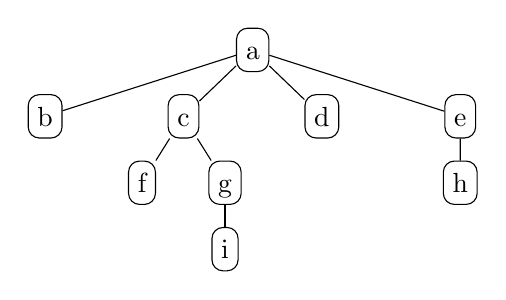
\begin{tikzpicture}
	[
		every node/.style = {
			shape=rectangle, rounded corners,
			draw, align=center
		},
		baseline,
		align=center,
		level distance=2\baselineskip,
		text depth=.1em,
		text height=.8em,
		level 1/.style={sibling distance=5em},
		level 2/.style={sibling distance=3em},
		level 3/.style={sibling distance=2em},
		level 4/.style={sibling distance=1em}
	]
	\node {a}
		child { node {b} }
		child { node {c}
			child { node {f} }
			child { node {g}
				child { node {i} }
			}
		}
		child { node {d} }
		child { node {e}
			child { node {h} }
		};
	\end{tikzpicture}
	\caption{An example of a tree for demonstration of representations.}
	\label{fig:tree}
\end{figure}

\section{Level-Order Unary Degree Sequence}

The first method of representing an ordinal tree succinctly was first described by \cite{jacobson1989space}.
The encoding of the tree is based on BFS traversal.
The vertices report their degrees in the unary system; we call it the \emph{degree sequence}
The representation is prefixed by \str{10}.

\begin{algorithm}
\begin{algorithmic}
\Function{\LOUDSRepresentation}{$R$}
	\State $Q \gets [\,]$%
	\Instr $\enqueue(Q, R)$ \Comment{The queue is initialized with the tree root.}
	\State $\out(\str{10})$
	\While{$V \gets \dequeue(Q)$}
		\ForAll{$C \gets \children(V)$}
			\State $\out(\str1)$
			\State $\enqueue(Q, C)$
		\EndFor
		\State $\out(\str0)$
	\EndWhile
\EndFunction
\end{algorithmic}
\end{algorithm}

\begin{lemma}
	There are $n$ ones and $n+1$ zeros in the LOUDS representation of a tree with $n$ vertices.
\end{lemma}
\begin{proof}
	The \str{10} corresponds to an artifical supervertex which has a single child -- the root of the tree.
	Each vertex of the tree is a child of a vertex and therefore was accounted by a one in the degree sequence of its parent.
	The number of ones is therefore the same as the number of all vertices in the tree.
	Each vertex is responsible for its own zero, plus there is one extra zero for the supervertex.
	
	The whole bit string, which we call $S$, has $N = 2n + 1$ bits.
\end{proof}

As there is a one and a zero belonging to each vertex, we can associate the $i$-th vertex with the $i$-th one and the $(i+1)$-th zero.
Note that the one is actually in the degree sequence of the parent of $i$, and the zero is terminating its degree sequence.
This follows from the the algorithm \LOUDSRepresentation{}: the $i$ vertex assigned one when it is added into the queue, and zero when its degree sequence is outputted.

We use the position of the associated one for the internal representation of a vertex.
A zeros-based structure is also possible as was showed by \cite{rahman2006engineering}.

\begin{example}
	The LOUDS representation of the tree in figure \ref{fig:tree} is:
	$$ S = \mathtt{\x1a \underline{0} \mid \x1b \x1c \x1d \x1e \underline{0} \mid 0 ~ \x1f \x1g 0 ~ 0 ~ \x1h \underline{0} \mid 0 ~ \x1i 0 ~ \underline{0} \mid \underline{0}} $$
	Levels are delimited by vertical bars, unary degree sequences of individual vertices by spaces.
	There is a vertex for each one.
	The underlined zeros are boundaries defined in section \ref{ss:louds-depth}.
\end{example}

\subsection{Navigation Operations}

We equip the bit string $S$ storing the representation of the tree with \rank{} and \select{} indices.
Because of the correspondence between ones and zeros, we can easily change between them using the following two functions.
The extra function \toBeginning{} returns the position where the degree sequence starts.

\begin{algorithm}
\begin{algorithmic}
\Function{\toOnes}{$S, i$}
	\State \Return{$\select_1(S, \rank_0(S, i) - 1)$}
\EndFunction
\end{algorithmic}
\end{algorithm}

\begin{algorithm}
\begin{algorithmic}
\Function{\toZeros}{$S, i$}
	\State \Return{$\select_0(S, \rank_1(S, i) + 1)$}
\EndFunction
\end{algorithmic}
\end{algorithm}

\begin{algorithm}
\begin{algorithmic}
\Function{\toBeginning}{$S, i$}
	\State \Return{$\select_0(S, \rank_1(S, i)) + 1$}
\EndFunction
\end{algorithmic}
\end{algorithm}

Only one vertex numbering schema is supported by this representation -- the level-order numbering.
The operations \loRank{} and \loSelect{} are simply $\rank_1(S, i)$ and $\select_1(S, r)$.


The navigation operations are relatively easy.
We also define an optimized version of the operation \childLast{} since we will need it later.

\begin{algorithm}
\begin{algorithmic}
\Function{\isRoot}{$S, i$}
	\State \Return{$i = 0$}
\EndFunction
\end{algorithmic}
\end{algorithm}

\begin{algorithm}
\begin{algorithmic}
\Function{\isLeaf}{$S, i$}
	\State \Return{$\toZeros(S, i) = \toBeginning(S, i)$} \Comment{Degree sequence is empty}
\EndFunction
\end{algorithmic}
\end{algorithm}

\begin{algorithm}
\begin{algorithmic}
\Function{\parent}{$S, i$}
	\State \Return{$\toOnes(S, \succ_0(S, i))$} \Comment{Conversion from zeros to ones}
\EndFunction
\end{algorithmic}
\end{algorithm}

\begin{algorithm}
\begin{algorithmic}
\Function{\degree}{$S, i$}
	\State \Return{$\toZeros(S, i) - \toBeginning(S, i)$} \Comment{Length of its degree sequence}
\EndFunction
\end{algorithmic}
\end{algorithm}

\begin{algorithm}
\begin{algorithmic}
\Function{\childRank}{$S, i$}
	\State \Return{$i - \pred_0(S, i)$} \Comment{Distance from the previous zero}
\EndFunction
\end{algorithmic}
\end{algorithm}

\begin{algorithm}
\begin{algorithmic}
\Function{\childSelect}{$S, i, k$}
	\State \Return{$\toBeginning(S, i) + k - 1$}
\EndFunction
\end{algorithmic}
\end{algorithm}

\begin{algorithm}
\begin{algorithmic}
\Function{\childLast}{$S, i$} \Comment{\childFirst{} is merely $\childSelect(S, i, 1)$.}
	\State \Return{$\toZeros(S, i) - 1$}
\EndFunction
\end{algorithmic}
\end{algorithm}

\bigbreak

The data structure can support more operations when augmented with more succinct indices.

\subsection{Depth and Level Queries}

We propose a new index for the LOUDS representation which allows us to query the depth of a vertex and which indirectly supports all level queries (without restriction on a subtree).
This was not possible before.

We call a \emph{level boundary} the terminal zero of the last vertex in each level, including the zero which belongs to the supervertex.
We define a bit string $D$ which contains $1$ at the position of level boundaries.

The bit string $D$ has size $N$ bits which does not make it a succinct index; we will discuss this in the next section.
We equip the bit string $D$ with succinct indices for \rank$_1$ and \select$_1$ which we described in the section \ref{s:op-bs}.

Using $D$, we can support \levelRank{}, \levelSelect{} and \levelSize{} (and thereby all \levelAny{} operations), and the operation \dep{}.

\begin{algorithm}
\begin{algorithmic}
\Function{\levelRank}{$S, i$}
	\State $z \gets \prev_1(D, i)$ \Comment{Terminal zero of the previous level}
	\State \Return{$\rank_1(S, i) - \rank_1(S, z)$}
\EndFunction
\end{algorithmic}
\end{algorithm}

\begin{algorithm}
\begin{algorithmic}
\Function{\levelSelect}{$S, i, l$}
	\State $z \gets \select_1(D, l)$ \Comment{Terminal zero of the previous level}
	\State \Return{$\select_1(S, \rank_1(S, z) + i)$}
\EndFunction
\end{algorithmic}
\end{algorithm}

\begin{algorithm}
\begin{algorithmic}
\Function{\levelSize}{$S, l$}
	\State $z \gets \select_1(D, l)$ \Comment{Terminal zero of the previous level}
	\State $z' \gets \select_1(D, l + 1)$ \Comment{Terminal zero of the next level}
	\State \Return{$\rank_1(S, z) - \rank_1(S, z')$}
\EndFunction
\end{algorithmic}
\end{algorithm}

\begin{algorithm}
\begin{algorithmic}
\Function{\dep}{$S, i$}
	\State \Return{$\rank_1(D, i)$}
\EndFunction
\end{algorithmic}
\end{algorithm}

\subsubsection{Succinct Index for Depth}\label{ss:louds-depth}

We cannot store the bit string $D$ directly, we cannot even store it as a FID.
If the tree has height $\Omega(n)$, then there is the same number of boundaries -- ones in the bit string $D$, which leads to $\Omega(N)$ bits from purely combinatorial reasons.

We work around the problem by utilizing the fact that if there are many levels, they must be short.
They are in fact short enough to precompute the level boundaries in a look-up table.

We split the bit string $D$ into blocks of size $b = \frac{\log N}{2}$; for each block $i$ we remember only the position of the first $1$, or lack thereof in a table $D'[i]$.
The table $D'$ requires $\frac{N}{b} \log b = O\left(\frac{N \log\log N}{\log N}\right) = o(N)$ bits.

\begin{lemma}
	Using the table $D'$, we can restore any block $i$ of $b$ consecutive bits of the original bit string $D$ in constant time.
\end{lemma}
\begin{proof}
	If there is no one in the block $i$, there is also no level boundary and the block contains only zeros.
	Otherwise, there is a $1$ at a position $p$.
	If $p = 2n$, then it is the last boundary which marks the end of the last level; the rest of the block is filled with zeros.

	From the properties of BFS it follows that the parent of the last vertex in a level is the last inner vertex in the previous level.
	An inner vertex contains $1$ in its degree sequence.
	By finding the last $1$ in the bit string $S$ before the boundary at position $p$, we find the last inner vertex in the previous level.
	Switching to the zero of its last child brings us to the position of the boundary $q$ for the level $i+1$.
	We iterate this process until we get out of the block.
	
	The crucial observation is that except for the first iteration, only bits from the block $i$ are needed.
	We can process the first iteration manually to obtain $q$ and then pass $p$ and $q$ to a look-up table \blockOfD{} which determines the rest of the boundaries within the block.
	Given the boundaries of a single level, the boundaries of the next level can be determined by counting the same number of zeros as there were ones in the previous level.
\end{proof}

\begin{algorithm}
\begin{algorithmic}
\Function{\blockOfD}{$S, i$} \Comment{$i$ is a block number.}
	\State $p' \gets D'[i]$
	\If{$p' = -1$} \Comment{No $1$ in the block}
		\State \Return{$0$}
	\Else
		\State $p \gets i b + p'$
		\If{$p = 2n$} \Comment{The end of the last level}
			\State \Return{$1 \bitlsh (b - p' - 1)$} \Comment{$1$ at position $p'$}
		\Else
			\State $q \gets \toZeros(S, \pred_1(S, p))$
			\If{$q \ge (i + 1) b $} \Comment{The level ends outsize of the block $i$.}
				\State \Return{$1 \bitlsh (b - p' - 1)$}
			\Else
				\State \Return{$\blockOfD[S[i b : (i + 1) b], p', q \% b]$}
			\EndIf
		\EndIf
	\EndIf
\EndFunction
\end{algorithmic}
\end{algorithm}

In a constant number of queries we can generate any $w$ bits of the original bit string $D$, which is the requirement for using the technique of an index without data from section \ref{ss:index-without-data}.

\subsection{\label{ss:leaf-queries}Leaf Operation}

Tree data structures often allow a direct iteration of their leaves.
Although the usual order of leaves corresponds to DFS traversal, LOUDS supports an access to the leaves in level-order in accordance with the its only ranking operation -- \loRank{}.
We also parametrize the operations by the desired depth of the leaves, by upper and lower bounds $u \le l$.

\begin{lemma}
	Whenever there are two consecutive zeros in the LOUDS representation, the latter one is associated with a leaf.
\end{lemma}
\begin{proof}
	There is always a zero immediately preceding the representation of every vertex.
	A leaf is a vertex with its degree equal to zero; the degree sequence consists of only a single zero.
	A leaf can therefore be localized by looking for two consecutive zeros; this gives us its zeros-based number.
\end{proof}

The original idea for this index comes from \cite{munro1998space}.
We have seen a solution to a similar problem in \ref{ss:index-without-data}.

We derive a bit string $L$ such that $L[i] = [S[i - 1] = 0 \booland S[i] = 0]$:
$$ L = \bitnot S \bitand \bitnot (S \bitrsh 1). $$
We build \rank{} and \select{} indices for it.

All the functions require a correction by one if the first vertex of the level $l$ is a leaf.

\begin{algorithm}
\begin{algorithmic}
\Function{\leafSize}{$S, l, u$}
	\State $f \gets \levelFirst(S, l)$ \Comment{The first vertex in the range}
	\State $f_0 \gets \toZeros(S, f)$
	\State $z_0 \gets \toZeros(S, \levelLast(S, u))$
	\State \Return $\rank_1(L, z_0) - \rank_1(L, f_0) + \isLeaf(S, f)$
\EndFunction
\end{algorithmic}
\end{algorithm}

\begin{algorithm}
\begin{algorithmic}	
\Function{\leafRank}{$S, l, i$} \Comment{We assume $i$ is a leaf at the admissible level.}
	\State $f \gets \levelFirst(S, l)$ \Comment{The first vertex in the range}
	\State $f_0 \gets \toZeros(S, f)$
	\State \Return{$\rank_1(L, \toZeros(i)) - \rank_1(L, f_0) + \isLeaf(S, f)$}
\EndFunction
\end{algorithmic}
\end{algorithm}

\begin{algorithm}
\begin{algorithmic}
\Function{\leafSelect}{$S, l, i$}
	\State $f \gets \levelFirst(S, l)$ \Comment{The first vertex in the range}
	\State $f_0 \gets \toZeros(S, f)$
	\State $o \gets \rank_1(L, f_0) - \isLeaf(S, f)$ \Comment{Offset}
	\State \Return{$\toOnes(S, \select_1(L, o + i))$}
\EndFunction
\end{algorithmic}
\end{algorithm}

\bigbreak

For the sake of completeness, we look at the other patterns:
\begin{description}
	\item[\str{01}]
	The symbol one in this pattern corresponds to the beginning of a degree sequence of an inner vertex (it has at least one child).
	\item[\str{10}]
	The symbol zero in this pattern corresponds directly to an inner vertex; its degree sequence contains at least one zero.
	\item[\str{11}]
	It is part of a degree sequence of vertices which have at least two children.
\end{description}

\subsection{Final Thoughts}

The main problem of the LOUDS representation appears to stem for the non-locality of the near vertices.
The unsupported operations are more concerned about ancestors and subtrees than siblings and levels.
We developed a new index for the operation \dep{} and \levelAny{} which greatly expands the possibilities.
Its simple implementation requiring only three types of indices (\rank{}, \select{}, \blockOfD{}) make it suitable for cases when there are not many requirements set on the supported operations.

\section{Balanced Parentheses}

In the previous section, we have seen that it is possible to build a succinct data structure for storing trees which requires essentially only the \rank{} and \select{} operations on the underlying bit string.
Here we focus on a different schema which exploits the property that the two symbols associated with a vertex are correctly matched in the bit string.
We represent them as parentheses in a balanced bit string, for which we utilize the \match{} and \enclose{} operations which we developed earlier in \ref{s:match-enclose}.

The representation is based on Depth-First Search and it follows two rules:
\begin{enumerate}
	\item When a vertex is entered from its parent, the vertex is \emph{opened} and an opening parenthesis is outputted in the representation.
	\item When the algorithm returns from a vertex to its parent, the vertex is \emph{closed} and a closing parenthesis is outputted.
\end{enumerate}
Although the root vertex does not have a parent, it is opened and closed as if it had one.

\begin{algorithm}
\begin{algorithmic}
\Function{\BPRepresentation}{$R$}
	\State $S \gets [\,]$%
	\Instr $\push(S, R)$ \Comment{The stack is initialized with the root of the tree.}
	\While{$V \gets \pop(S)$}
		\If{$V.\state = \UNSEEN$} \Comment{We came from its parent.}
			\State $\push(S, V)$ \Comment{We return $V$ to the stack.}
			\State $V.\state \gets \OPEN$
			\State $\out(\openingParen)$
			\ForAll{$C \in \reverse(\children(V))$}
				\State $\push(S, C)$
			\EndFor
		\ElsIf{$V.\state = \OPEN$} \Comment{All children has been processed.}
			\State $V.\state \gets \CLOSED$
			\State $\out(\closingParen)$
		\EndIf
	\EndWhile
\EndFunction
\end{algorithmic}
\end{algorithm}

In the algorithm, the $\reverse$ is needed only to maintain the order of children.

An alternative definition of this schema can be expressed recursively:
\begin{enumerate}
	\item A leaf is encoded with a pair of parentheses.
	\item An inner vertex is encoded as a concatenated string of encodings of its children surrounded by a pair of parentheses.
\end{enumerate}
We can see from this definition that each subtree forms a continuous substring.

We associate each vertex with its opening parenthesis.
By using the operation \match{} we can easily switch between these two.

\begin{example}
	The BP representation of the tree in figure \ref{fig:tree} including vertex association is:
	$$ S = \mathtt{ \x(a \x(b) ~ \x(c \x(f ) \x(g \x(i) ) ) ~ \x(d) ~ \x(e \x(h) ) ) }$$ 
	The spaces separate representations of children of the root $a$.
\end{example}

\bigbreak

The operations \preRank{}, \preSelect{}, \postRank{}, and \postSelect{} are immediately supported by opening-based and closing-based \rank{}s and \select{}s on the underlying bit string $S$.
We first show implementation of the operations which do not need any auxiliary index and which can be expressed using only the primitives provided by $S$.

\begin{algorithm}
\begin{algorithmic}
\Function{\isRoot}{$S, i$}
	\State \Return{$i = 0$}
\EndFunction
\end{algorithmic}
\end{algorithm}

\begin{algorithm}
\begin{algorithmic}
\Function{\isLeaf}{$S, i$}
	\State \Return{$S[i + 1] = \closingParen$} \Comment{Is the parenthesis immediately closed?}
\EndFunction
\end{algorithmic}
\end{algorithm}

\subsection{Navigation Operations}

\begin{algorithm}
\begin{algorithmic}
\Function{\parent}{$S, i$}
	\State \Return{$\enclose(S, i)$}
\EndFunction
\end{algorithmic}
\end{algorithm}

Neither \degree{} nor \childRank{} nor \childSelect{} are available without an additional index; we therefore resort to the direct implementation of the rest of the \childAny{} operations:

\begin{algorithm}
\begin{algorithmic}
\Function{\childFirst}{$S, i$}
	\State \Return{$i + 1$}
\EndFunction
\end{algorithmic}
\end{algorithm}

\begin{algorithm}
\begin{algorithmic}
\Function{\childLast}{$S, i$}
	\State \Return{$\findOpen(\findClose(S, i) - 1)$}
\EndFunction
\end{algorithmic}
\end{algorithm}

\begin{algorithm}
\begin{algorithmic}
\Function{\childNext}{$S, i$}
	\State \Return{$\findClose(S, i) + 1$}
\EndFunction
\end{algorithmic}
\end{algorithm}

\begin{algorithm}
\begin{algorithmic}
\Function{\childPrev}{$S, i$}
	\State \Return{$\findOpen(S, i - 1)$}
\EndFunction
\end{algorithmic}
\end{algorithm}

\subsection{Other Native Operations}\label{ss:bp-other}

The following natively supported operations use the property that a subtree of $v$ is fully contained in the representation of $v$.

\begin{algorithm}
\begin{algorithmic}
\Function{\dep}{$i$}
	\State \Return{$\parenDepth(i)$}
\EndFunction
\end{algorithmic}
\end{algorithm}

\begin{algorithm}
\begin{algorithmic}
\Function{\isAncestor}{$i_1, i_2$}
	\State \Return{$i_1 \le i_2 \booland \findClose(i_1) \ge i_2$}
\EndFunction
\end{algorithmic}
\end{algorithm}

\begin{algorithm}
\begin{algorithmic}
\Function{\subtreeSize}{$i$}
	\State \Return{$\rank_((\findClose(i)) - \rank_((i) + 1$}
\EndFunction
\end{algorithmic}
\end{algorithm}

The group of operations consisting of \lca{}, \distance{}, \deepestVertex{}, and \hei{} can be solved by \enclose{} and maximum range queries.

\begin{algorithm}
\begin{algorithmic}
\Function{\lca}{$i_1, i_2$}
	\If{$\isAncestor(i_1, i_2)$}
		\State \Return{$i_1$}
	\ElsIf{$\isAncestor(i_2, i_1)$}
		\State \Return{$i_2$}
	\Else
		\State \Return{$\enclose(i_1, i_2)$}
	\EndIf
\EndFunction
\end{algorithmic}
\end{algorithm}

\begin{algorithm}
\begin{algorithmic}
\Function{\distance}{$i_1, i_2$}
	\State $a \gets \lca(i_1, i_2)$
	\State \Return{$\dep(i_1) + \dep(i_2) - 2 \dep(a)$}
\EndFunction
\end{algorithmic}
\end{algorithm}

\begin{algorithm}
\begin{algorithmic}
\Function{\deepestVertex}{$i$}
	\State \Return{$\RMQi(i, \match(i))$}
\EndFunction
\end{algorithmic}
\end{algorithm}

\begin{algorithm}
\begin{algorithmic}
\Function{\hei}{$i$}
	\State \Return{$\dep(\deepestVertex(i)) - \dep(i)$}
\EndFunction
\end{algorithmic}
\end{algorithm}

\subsection{In-Order Rank and Select and Leaf Operations}

An in-order number is assigned to a vertex for each two children in a row.
This situation can be detected in the bit string $S$ by searching for the pattern \str{)(}, which means that one vertex ends and its right sibling starts.
Each occurrence of the pattern is accounted as an in-order number being assigned to their parent.

We recall how the parentheses are actually stored: \openingParen = 1, \closingParen = 0.
With that in our mind, we derive a bit string $I$ which contains $1$ at the position of the opening parenthesis which is preceded by a closing parenthesis: $I[i] = [S[i] = 1\allowbreak \booland S[i-1] = 0]$:
$$ I = \bitnot S \bitand (S \bitrsh 1). $$
The operations \inRank{} and \inSelect{} are then defined on this derived bit string.

Note that the operation \inRank{} returns the smallest assigned in-order number, and that \inSelect{} find the vertex by any in-order number which it has been assigned.
Also, we cannot use the operation \degree{} in the implementation since it is not supported.

\begin{algorithm}
\begin{algorithmic}
\Function{\inRank}{$S, i$}
	\If{$\isLeaf(S, i) \boolor \childFirst(S, i) = \childLast(S, i)$}
		\State \Return{$-1$}
	\Else
		\State \Return{$\rank_1(I, \childFirst(S, i))$}
	\EndIf
\EndFunction
\end{algorithmic}
\end{algorithm}

\begin{algorithm}
\begin{algorithmic}
\Function{\inSelect}{$S, r$}
	\State $s \gets \select_1(I, r)$
	\If{$s = N$} \Comment{\select{} is out of range; we need an explicit check.}
		\State \Return{$-1$}
	\Else
		\State \Return{$\parent(S, s)$}
	\EndIf
\EndFunction
\end{algorithmic}
\end{algorithm}

\bigbreak

We us a similar technique as in \ref{ss:leaf-queries} to support the leaf operations, this time restricted to a subtree rather than a level.
A vertex is a leaf if its opening parenthesis is immediately closed.
We are looking for a pattern \str{()}, for which we derive a bit string $L$ such that $L[i] = [S[i] = 1 \booland S[i+1] = 0]$:
$$L = S \bitand (\bitnot S \bitlsh 1). $$

\begin{algorithm}
\begin{algorithmic}
\Function{\leafSize}{$S, a$}
	\If{$\isLeaf(a)$}
		\State \Return{$1$}
	\Else
		\State \Return{$\rank_1(L, \findClose(a)) - \rank_1(L, a)$}
	\EndIf
\EndFunction
\end{algorithmic}
\end{algorithm}

\begin{algorithm}
\begin{algorithmic}	
\Function{\leafRank}{$S, a, i$} \Comment{We assume $i$ is in the subtree of $a$.}
	\If{$\isLeaf(a)$}
		\State \Return{$1$}
	\Else
		\State \Return{$\rank_1(L, i) - \rank_1(L, a)$}
	\EndIf
\EndFunction
\end{algorithmic}
\end{algorithm}

\begin{algorithm}
\begin{algorithmic}
\Function{\leafSelect}{$S, a, i$}
	\If{$\isLeaf(a)$}
		\State \Return{$a$}
	\Else
		\State \Return{$\select_1(L, \rank_1(L, a) + i)$}
	\EndIf
\EndFunction
\end{algorithmic}
\end{algorithm}

\bigbreak

We may be interested in the two other patterns:
\begin{description}
	\item[\str{((}]
	If we focus on the first symbol of the pattern, it corresponds to a vertex which has a child.
	We could therefore derive similar operations to \leafAny{} which would be defined for inner vertices.
	
	The second symbol corresponds to the first child of an inner vertex; which can also be obtained by \childFirst{} operation applied to its parent.
	
	\item[\str{))}]
	Again, it can be used to query inner vertices or last children.
	It is less useful, since the same can be done by the previous pattern without the need of an extra call of \findOpen{}.
\end{description}

\subsection{Final Thoughts}

Three more indices have been developed for the BP representation:
\begin{description}
	\item[\degree{}]
	An index by \cite{chiang2005orderly}.

	\item[\childRank{}, \childSelect{}]
	An index by \cite{lu2008balanced}.
	Together with the index for \degree{}, the indices complete the set of navigation operation and make the structure useful for a wider set of use cases.

	\item[\levelAncestor{}, \levelPrev{}, \levelNext{}]
	An index by \cite{munro2012succinct}.
\end{description}
We did not show these indices as they are rather complicated.
We are going to show in the next chapter a different structure based on the same BP representation, which supports all these operations (including \levelAny{}) natively.

The operations which remain unsupported are:
\begin{iteminline}
	\item \levelAny{} operations (only \levelPrev{}, \levelNext{} are supported);
	\item \dfudsRank{} and \dfudsSelect{} (that is the numbering schema which is native to the representation that we introduce next).
\end{iteminline}

Its main advantage of the BP representation is the simplicity and the support for many operations including \lca{} and the \dep{}, for which it pays by hard, yet not impossible, \childRank{}, \childSelect{} and \degree{} operations.
If we restrict degrees of the vertices to constants, the BP representation suddenly becomes a very good choice.

\section{Depth-First Unary Degree Sequence}

The \emph{Depth-First Unary Degree Sequence} (DFUDS) is an encoding which tries to combine the advantages from both LOUDS (child queries are natively supported) and BP (each subtree is stored locally instead of being spread throughout the encoding).
It was originally proposed by \cite{benoit1999representing}.

The encoding is defined recursively:
\begin{enumerate}
	\item A leaf is encoded as a closing parenthesis.
	\item An inner vertex is encoded as $\degree$ opening parentheses followed by a single closing parenthesis (which we again call the \emph{degree sequence}) and concatenated encodings of its children.
\end{enumerate}
For convenience, one opening parenthesis is prepended to make the sequence of parentheses balanced.

\begin{algorithm}
\begin{algorithmic}
\Function{\DFUDSRepresentation}{$R$}
	\State $S \gets [\,]$%
	\Instr $\push(S, R)$ \Comment{The stack is initialized with the root of the tree.}
	\State $\out(\openingParen)$
	\While{$V \gets \pop(S)$}
		\ForAll{$C \gets \reverse(\children(V))$}
			\State $\out(\openingParen)$
			\State $\push(S, C)$
		\EndFor
		\State $\out(\closingParen)$
	\EndWhile
\EndFunction
\end{algorithmic}
\end{algorithm}

\begin{lemma}\label{l:dfuds}
	The DFUDS encoding provides a balanced bit string.
\end{lemma}
\begin{proof}
	When we prepend an opening parenthesis in front of an encoding of any subtree, we obtain a balanced bit string.
	
	The proof goes by induction on height of a subtree.
	The claim holds for a leaf, which is only a closing parenthesis, which misses its matching opening one.
	
	We assume, that the claim holds for all $d = \degree(v)$ subtrees $T_1, \ldots, T_d$ of a vertex $v$.
	The degree sequence of the vertex $v$ contains $d$ opening and one closing parenthesis.
	The closing one matches the last opening one within the degree sequence, and $d - 1$ of them are left to be matched with the excessive parentheses in the subtrees.
	All parentheses in $T_1, \ldots, T_{d-1}$ get matched, leaving one closing parenthesis in $T_d$ unmatched, which is the one that the claim requires.
	
	The only unmatched parenthesis of the representation of the whole tree is matched in the end with the artificially prepended one.
\end{proof}

We associate each vertex with the first symbol of its representation.
Alternatively, we can associate it with the terminal zero of its degree sequence (we will indeed define functions that switch between them).
The association with the opening parenthesis in the degree sequence of its parent (similar to LOUDS) is also possible as we show later by defining \dfudsRank{} and \dfudsSelect{}.

\begin{example}
	The DFUDS representation of the tree in figure \ref{fig:tree} including vertex association is:
	$$ S = \mathtt{( ~ \x(a((() ~ \x)b ~ \x(c() ~ \x)f ~ \x(g) ~ \x)i ~ \x)d ~ \x(e) ~ \x)h }$$ 
	The spaces separate the unary degree sequences of the vertices.
\end{example}

\subsection{Navigation Operations}

It is easy to test whether a vertex is the root or a leaf.

\begin{algorithm}
\begin{algorithmic}
\Function{\isRoot}{$S, i$}
	\State \Return{$i = 1$} \Comment{Mind the artificially prepended parenthesis.}
\EndFunction
\end{algorithmic}
\end{algorithm}

\begin{algorithm}
\begin{algorithmic}
\Function{\isLeaf}{$S, i$}
	\State \Return{$S[i] = \closingParen$} \Comment{Is the parenthesis a closing one?}
\EndFunction
\end{algorithmic}
\end{algorithm}

The crucial observations for the following operations are:
\begin{enumerate}
	\item The representation of a vertex is preceded by a closing parenthesis with the exception of the root.
	\item The opening parenthesis in the degree sequence matches the closing parenthesis immediately preceding the representation of a child.
	\item In a subtree of a vertex $v$, the last closing parenthesis, which represents the last leaf, matches a parenthesis in the degree sequence of the parent of $v$.
\end{enumerate}
The observations follow from the same induction as in lemma \ref{l:dfuds}.

\bigbreak

We first define two helper functions which navigate from any position in a vertex degree sequence to its beginning (which is the symbol associated with the vertex) and to its end (which is always a closing parenthesis).
We also define a function which navigates to the last parenthesis of the vertex representation.

\begin{algorithm}
\begin{algorithmic}
\Function{\toBeginning}{$S, p$}
	\If{$p = 0$}
		\State \Return{$-1$} \Comment{The representation of the root starts at position $1$.}
	\ElsIf{$\prev_)(S, p) < 0$}
		\State \Return{$1$} \Comment{Correction for the root}
	\Else
		\State \Return{$\prev_)(S, p) + 1$}
	\EndIf
\EndFunction
\end{algorithmic}
\end{algorithm}

\begin{algorithm}
\begin{algorithmic}
\Function{\toEnd}{$S, p$}
	\If{$p = 0$}
		\State \Return{$-1$}
	\Else
		\State \Return{$\succ_)(S, p)$}
	\EndIf
\EndFunction
\end{algorithmic}
\end{algorithm}

\begin{algorithm}
\begin{algorithmic}
\Function{\toLast}{$S, p$}
	\If{$\isLeaf(S, p)$}
		\State \Return{$p$}
	\Else
		\State \Return{$\findClose(S, \enclose(S, \toBeginning(S, p)))$}
	\EndIf
\EndFunction
\end{algorithmic}
\end{algorithm}

The navigation operations can be immediately defined.

\begin{algorithm}
\begin{algorithmic}
\Function{\parent}{$S, i$}
	\State $p \gets \findOpen(S, i - 1)$ \Comment{Inside parent's degree sequence}
	\State \Return{$\toBeginning(S, p)$}
\EndFunction
\end{algorithmic}
\end{algorithm}

\begin{algorithm}
\begin{algorithmic}
\Function{\degree}{$S, i$}
	\State \Return{$\toEnd(S, i) - i$}
\EndFunction
\end{algorithmic}
\end{algorithm}

\begin{algorithm}
\begin{algorithmic}
\Function{\childRank}{$S, i$}
	\State $p \gets \findOpen(S, i - 1)$
	\State \Return{$\toEnd(S, p) - p$}
\EndFunction
\end{algorithmic}
\end{algorithm}

\begin{algorithm}
\begin{algorithmic}
\Function{\childSelect}{$S, i, k$}
	\State $p \gets \toEnd(S, i) - k$
	\State \Return{$\findClose(S, p) + 1$}
\EndFunction
\end{algorithmic}
\end{algorithm}

\subsection{Other Native Operations}

\begin{algorithm}
\begin{algorithmic}
\Function{\preRank}{$S, i$}
	\State \Return{$\rank_)(S, \toEnd(S, i))$}
\EndFunction
\end{algorithmic}
\end{algorithm}

\begin{algorithm}
\begin{algorithmic}
\Function{\preSelect}{$S, r$}
	\State \Return{$\toBeginning(S, \select_)(S, i))$}
\EndFunction
\end{algorithmic}
\end{algorithm}

In order to support \dfudsRank{} and \dfudsSelect{}, we will need another helper function \toSymmetric{} which navigates from $k$-th opening parenthesis in the degree sequence of vertex $v$ to $(\degree(v) - k - 1)$-th one.

\begin{algorithm}
\begin{algorithmic}
\Function{\toSymmetric}{$S, p$}
	\State $b \gets \toBeginning(S, p)$
	\State \Return{$b + \degree(S, b) - (p - b) - 1$}
\EndFunction
\end{algorithmic}
\end{algorithm}

\begin{algorithm}
\begin{algorithmic}
\Function{\dfudsRank}{$S, i$}
	\If{$\isRoot(S, i)$}
		\State \Return{$1$}
	\Else
		\State $p \gets \findOpen(S, i - 1)$
		\State \Return{$\rank_((S, \toSymmetric(S, p))$}
	\EndIf
\EndFunction
\end{algorithmic}
\end{algorithm}

\begin{algorithm}
\begin{algorithmic}
\Function{\dfudsSelect}{$S, r$}
	\If{$r = 1$}
		\State \Return{$1$}
	\Else
		\State $p \gets \toSymmetric(S, \select_((S, r))$
		\State \Return{$\findClose(S, p) + 1$}
	\EndIf
\EndFunction
\end{algorithmic}
\end{algorithm}

And finally there are two simple subtree-oriented operations which use the helper function \toLast{}.

\begin{algorithm}
\begin{algorithmic}
\Function{\isAncestor}{$i_1, i_2$}
	\If{$\isLeaf(i_1)$}
		\State \Return{$i_1 = j_2$}
	\Else
		\State \Return{$i_1 \le i_2 \le \toLast(S, i_1)$}
	\EndIf
\EndFunction
\end{algorithmic}
\end{algorithm}

\begin{algorithm}
\begin{algorithmic}
\Function{\subtreeSize}{$i$}
	\If{$\isLeaf(S, i)$}
		\State \Return{$1$}
	\Else
		\State \Return{$\rank_)(S, \toLast(S, i)) - \rank_)(S, i)$}
	\EndIf
\EndFunction
\end{algorithmic}
\end{algorithm}

\subsection{Lowest Common Ancestor}

The operation LCA is surprisingly similar to the one for BP \ref{ss:bp-other}, however it needs to be shown.
The proof is by \cite{fischer2010optimal}.

Let's assume that neither $i_1$ nor $i_2$ is an ancestor of the other one; in that case $\min(i_1, i_2)$ would be the answer.
We further assume that $i_1 < i_2$ and that their lowest common ancestor is $j = \lca(i_1, i_2)$.
The vertex $j$ is the smaller from both $i_1, i_2$ because it is assigned a lower pre-order number than any of its descendants.
We call (like in section \ref{ss:enclose2}) $p_1 < p_2$ the distinct children of $j$ whose subtrees contain $i_1$ and $i_2$.

We look at excess values of children of $j$.
Each child and its subtree forms a sequence of matching parentheses with the exception of the last one, which is a closing parenthesis and stays unmatched (lemma \ref{l:dfuds}).
From this, it follows that $\rmqi(S, i, \toLast(S, i)) = \toLast(S, i)$.

We look into the properties of $\rmqi(S, i_1, i_2 - 1)$.
The last parenthesis of the representation of a child $c$ of the vertex $j$ which is contained in the range sets a new minimum.
There may be an issue with the subtree of $p_2$, which is not fully contained in the range.
If it contained the minimum elsewhere, then we cannot simply navigate to the vertex $j$.

It cannot be the last parenthesis of $p_2$, because we end the interval just before it.
It also will not be any other parenthesis $p \ge p_2$:
\begin{align*}
	& \excess(S, \toLast(S, p_2)) + 1 \\
	&\quad = \excess(S, \toLast(S, \childPrev(S, p_2))) \\
	&\quad \le \excess(S, p).
\end{align*}
In case of equality, the \rmqi{} returns the leftmost occurrence.

The $\rmqi(S, i_1, i_2 - 1)$ returns position of the last parenthesis of the previous sibling of $p_2$ and therefore $p_2 = \rmqi(S, i_1, i_2 - 1) + 1$.
The result is then $\lca(S, i_1, i_2) = j = \parent(S, p_2)$.

\begin{algorithm}
\begin{algorithmic}
\Function{\lca}{$i_1, i_2$}
	\If{$\isAncestor(i_1, i_2)$}
		\State \Return{$i_1$}
	\ElsIf{$\isAncestor(i_2, i_1)$}
		\State \Return{$i_2$}
	\Else
		\State $p_2 \gets \rmqi(i_1, i_2 - 1) + 1$
		\State \Return{$\parent(p_2)$}
	\EndIf
\EndFunction
\end{algorithmic}
\end{algorithm}

\subsection{Leaf operations}

The operations on leaves can be defined similarly to those for the LOUDS and BP representation.
We are looking for the second of two consecutive closing parentheses -- \str{))}.
This follows from the property that the degree sequence of every vertex is preceded by a closing parenthesis, and the degree sequence of leaves is only the closing parenthesis.
Note that this does not work in case when the tree root is a leaf, however this special case is easy to handle, too.

The other patterns are the same as in case of the LOUDS representation in section \ref{ss:leaf-queries}.

\subsection{Final Thoughts}

Two indices were proposed to extend the set of supported operations beyond what we have shown.
\begin{description}
	\item[\dep{}]
	An index by \cite{jansson2012ultra}.
	Supporting the operation \dep{} makes also possible to query \distance{} between vertices.
	
	\item[\levelAncestor{}]
	An index also by \cite{jansson2012ultra}.
\end{description}

DFUDS is the opposite of BP: it is less intuitive, it supports all the basic navigation queries, however it lacks an easy support for the \dep{} operation.
It is a good choice if the \preRank{} and \childAny{} operations are important for the use case.